\chapter{Estado del Arte}
\label{chap:ea}
Este capítulo se centra en detallar el estado actual de las tecnologías utilizadas en el proyecto así como en analizar soluciones similares al proyecto.
\section{Visualización}
Los componentes artificiales que deseamos incluir en las imágenes del mundo real proceden del framework desarrollado por \citeauthor{Kroes2012} que aplica técnicas de \acrfull{mcrt} sobre \acrfull{dvr}.

El termino \acrshort{dvr} se utiliza para referirse a las técnicas que producen una imagen directamente a partir de datos de un volumen, sin realizar pasos intermedios. Para que esto sea posible es necesario implementar modelos físicos que indiquen cómo se genera, refleja, dispersa o oculta la luz \cite{Max1995}. Estos modelos con el paso del tiempo han evolucionado en modelos más y más complejos que han probado ser beneficiosos para la visualización científica de modelos 3D \cite{Daz2015}, \cite{Englund2016}, \cite{Lindemann2011} .

La implementación de estos modelos conlleva altos tiempos de renderizado, o en su defecto, un equipo increíblemente costoso para poder obtener una experiencia interactiva \cite{IglesiasGuitian2022}. Para enfrentar esta casuística,  \citeauthor{IglesiasGuitian2022} implementan un algoritmo de reducción de ruido basado en \acrfull{rls} que permite una experiencia interactiva en tiempo real, sobre \acrshort{gpu}s comerciales. Este proyecto se fundamenta en \cite{IglesiasGuitian2022} para el renderizado de las imágenes que posteriormente se apliquen en realidad aumentada sobre las imágenes reales.

\section{Realidad Extendida}

Para llevar a cabo el proyecto existen varias aproximaciones en el estado del arte \cite{Venkatesan2021}.Se seleccionaron aquellas que más se ajustaban al proyecto.
Uno de los objetivos principales es el seguimiento de piezas extraídas de un \acrshort{tc} y diseñar marcadores que facilitasen el registro de las mismas, por lo que se optó por un seguimiento basado en marcadores. No obstante, en lo que a la visualización se refiere, es necesario un equipo con gran potencia computacional, o en su defecto, un visor que permita la reproducción de vídeo renderizado por un tercer equipo. Dadas estas restricciones se decidió por utilizar un \acrfull{hmd} HTC VIVE PRO. Utilizando la \figurename~\ref{fig:vrAproximations} \cite{Venkatesan2021} como referencia , el sistema implementado se compondría de un seguimiento basado en marcadores (E) visualizando estos marcadores en realidad aumentada (B).
Para este proyecto se escogieron las tecnologías E y G que se observan en  la \figurename~\ref{fig:vrAproximations}

\begin{figure}
  \centering
  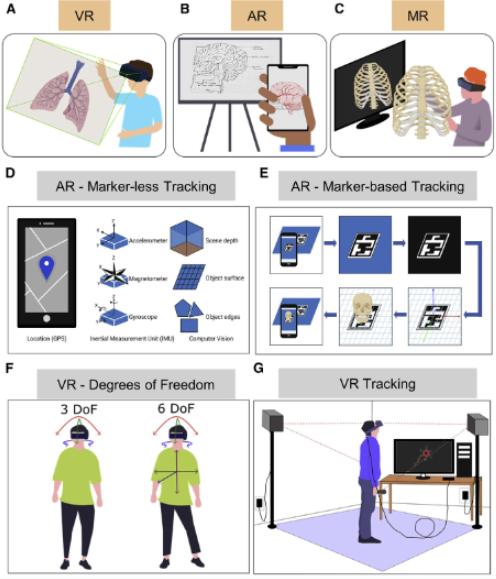
\includegraphics[width=0.75\textwidth]{imaxes/aproxVR.png}
  \caption{Aproximaciones a la realidad extendida para aplicaciones biomédicas.(fuente: \cite{Venkatesan2021})}
  \label{fig:vrAproximations}
\end{figure}

Destacar también la solución presentada por \cite{MoretaMartinez2020}. Este proyecto presenta un método para diseñar aplicaciones de realidad aumentada para la visualización de modelos anatómicos en 3 dimensiones mediante el uso de un marcador fiduciario. En el se explica un método para extraer una figura a partir de una \acrshort{tc}. Posteriormente, provee instrucciones detalladas para la impresión 3D del marcador fiduciario. Finalmente utilizando la extensión de Vuforia para Unity crea una aplicación móvil que permite la visualización en realidad aumentada de la pieza. 

\section{Impresión 3D}
La impresión 3D o fabricación aditiva es un proceso para manufacturar objetos de cualquier forma o tamaño a partir de un modelo 3D o otro tipo de fuente electrónica a partir de procesos aditivos en los que sucesivas capas de material se depositan bajo control de un ordenador \cite{yan_dong_su_han_song_wei_shi_2018}.
Desde 1984 \cite{ChanaRodrguez2016} hasta la actualidad, la impresión 3D ha afrontado una revolución que se fundamenta en pilares sólidos como el abaratamiento de los costes de producción de impresoras 3D, la mejora de su precisión y velocidad, el software libre, la comercialización de los productos a usuarios finales , documentación, formación extensa corroborada y creada por terceros que facilita y realimenta el desarrollo de nuevos proyectos.
Producto de esto, ha sido la implementación de esta tecnología en el ámbito sanitario, tanto para la producción de herramientas especializadas \cite{ChanaRodrguez2016} como para el diseño y la implantación de prótesis personalizadas para cada paciente \cite{Gonzalez_Alvarez_2021}.
